\documentclass[11pt,a4paper]{article}
\usepackage[T1]{fontenc}
\usepackage[margin=2.3cm]{geometry}
\usepackage{amsmath,amssymb}
\usepackage{graphicx}
\usepackage[dvipsnames]{xcolor}
\usepackage{enumitem}
\usepackage[colorlinks=true,linkcolor=blue,urlcolor=blue]{hyperref}
\setlength{\parskip}{0.6em}
\setlength{\parindent}{0pt}
\begin{document}

\begin{center}{\LARGE\bfseries openboiling}\\[0.4em]{\large Model boiling and bubble growth on a heated surface, in three sessions.}\\[0.2em]\small PAN IIT OSS explainer \textbullet{} higher secondary to diploma / undergraduate (levels 4-5)\end{center}

\section*{Why this exists}
A hot surface under water can carry away enormous amounts of heat by boiling, until a limit is crossed and a vapour film suddenly insulates it. This explainer shows the energy balance, the boiling curve and the burnout using only simple equations, so you can build the model yourself.

\section*{The end goal}
Model boiling and bubble growth on a heated surface. The end goal is to model boiling and bubble growth on a heated surface: the boiling curve, the critical heat flux and the growth of a bubble. The same ideas matter in power plants, electronics cooling and the quenching of hot metal, always with large safety margins and real validated data.

\section*{How the three sessions build up}
\begin{enumerate}[nosep]
\item \textbf{Session 1: Why a pot of water gets stuck at 100 C} (Level 1, conceptual interactive model, 60 min).
\item \textbf{Session 2: Energy to boil, heat flux and the limits of a heater} (Level 2, mathematical engineering model, 75 min).
\item \textbf{Session 3: A heated plate, the burnout and the growing bubble} (Level 3, simulation and validation, 90 min).
\end{enumerate}

\section{Session 1: Why a pot of water gets stuck at 100 C}

\subsection*{A. Real-world problem}
You put a pot of water on the stove. For a few minutes it just gets warmer. Then bubbles appear at the bottom and the temperature stops rising, although the heater still pours energy in. Where does the energy go? And why do bubbles start on the hot surface, not in the middle of the water? (General education only: this is not advice for operating real heating equipment.)

\subsection*{B. Concept and theory}
Heat is energy, measured in joules (J); power is energy per second, in watts (W). Warming m kilograms of water by a temperature difference dT needs m cp dT, where cp = 4186 J/(kg K) is how much energy 1 kg needs for 1 K. At the boiling point (100 C at normal air pressure) extra energy L = 2.257 million J per kilogram is needed to turn the water into steam; the water stays at 100 C while this happens. Bubbles form on the heater surface because the water touching the metal is hotter than the water further away. Now imagine holding the metal at dT kelvin above the boiling point and measuring the heat flux q, in watts per square metre, leaving it. The boiling curve plots q against dT and has four stages: natural convection (no bubbles), nucleate boiling (bubbles, very steep rise), the critical heat flux followed by transition boiling (flux falls), and film boiling (a vapour blanket insulates the surface).

\begin{itemize}[nosep]
\item m: mass of water (kg)
\item cp: specific heat of liquid water (4186) (J/(kg K))
\item L: latent heat of vaporisation (2.257e6) (J/kg)
\item P: heater power (W)
\item eta: fraction of power reaching the water (0.85) (no unit)
\item dT: surface temperature above the boiling point (K)
\item q: heat flux leaving the surface (W/m2)
\end{itemize}

\begin{equation*}
t_{\mathrm{boil}}=\frac{m\,c_p\,(100-T_0)}{\eta\,P}
\end{equation*}

\begin{equation*}
\dot m_{\mathrm{steam}}=\frac{\eta\,P}{L}\qquad(\text{once the water is at }100\,^\circ\mathrm{C})
\end{equation*}

\begin{equation*}
q=\frac{\text{heat leaving the surface}}{\text{area}}\quad[\mathrm{W/m^2}]
\end{equation*}

\begin{center}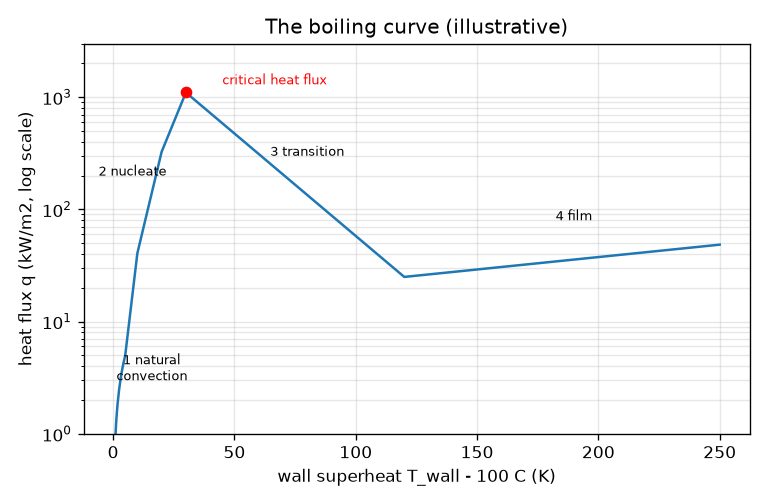
\includegraphics[width=0.85\linewidth]{figures/s01_boiling_curve_levels.png}\\\small The boiling curve with its four stages and the critical heat flux (illustrative numbers).\end{center}

\subsection*{E. Worked example}
1 kg of water at 20 C on a 2000 W heater with efficiency 0.85. When does it boil, and how much water has boiled away 5 minutes later?
\begin{enumerate}[nosep]
\item Energy to warm it: m cp dT = 1 * 4186 * 80 = 334 880 J.
\item Useful power: 0.85 * 2000 = 1700 W.
\item Time to boil: 334 880 / 1700 = 197 s (3 minutes 17 seconds).
\item During the next 300 s the energy is 1700 * 300 = 510 000 J, all of it making steam.
\item Mass boiled away: 510 000 / 2.257e6 = 0.226 kg.
\end{enumerate}
\textbf{Answer.} It boils after 197 s; 5 minutes later it is still at 100 C and 226 g (22.6 percent) has boiled away.

\subsection*{F. Questions}
\begin{enumerate}[nosep]
\item \textbf{Conceptual.} The heater keeps delivering 2000 W once the water is boiling, yet the temperature stays at 100 C. Where does the energy go?
\item \textbf{Numerical.} 1.5 kg of water at 20 C on an 1800 W heater (efficiency 0.85). How long until it boils, and how much boils away in the next 2 minutes?
\item \textbf{Graph and simulation interpretation.} On the boiling curve, compare the heat flux of a surface 10 K above boiling, one 60 K above and one 200 K above. Name the stage of each. What is surprising?
\item \textbf{Design and optimisation challenge.} Design: choose a heater power so that 1 litre (1 kg) of water boils in 3 minutes from 20 C, then say how much water you lose in 10 minutes if you leave it at that power. Suggest a better way to keep it boiling.
\end{enumerate}

\section{Session 2: Energy to boil, heat flux and the limits of a heater}

\subsection*{A. Real-world problem}
An electric kettle must bring 1.7 kg of water to the boil in four minutes. How many watts is that? Once we know the power, how hot does the metal element get above the water, how close is it to the critical heat flux (where boiling stops working and the surface overheats), and how big must the element be to stay safely away from it? (Simplified model; real kettles need certified safety design and boil-dry protection.)

\subsection*{B. Concept and theory}
The energy to bring m kilograms from T0 to the boiling point is m cp (100 - T0); boiling away a mass m\_s needs m\_s L. The heating time at electrical power P and efficiency eta is the energy divided by eta P. The heat flux through the element is q = eta P / A. A heat transfer coefficient h is defined by q = h dT, where dT = T\_wall - T\_sat is the wall superheat. In nucleate boiling h is not constant: an EMPIRICAL SCALING of Rohsenow type says q is proportional to dT cubed, so h grows as dT squared. The exponent is typically between about 2.5 and 4 in published data (3 is the usual textbook value), and the coefficient varies by factors of several with surface material, roughness and cleanliness, so the exponent is the robust part and the coefficient is not. Nucleate boiling has an upper limit, the critical heat flux (CHF): Zuber's estimate for a large flat plate is q\_chf = 0.131 L sqrt(rho\_v) (sigma g (rho\_l - rho\_v))\textasciicircum{}(1/4), about 1.1 MW/m2 for water at normal pressure (the commonly quoted round figure is about 1 MW/m2; it is an approximate value). Bubble size is set by buoyancy against surface tension: the capillary length sqrt(sigma / (g (rho\_l - rho\_v))) is about 2.5 mm for water at 100 C and Fritz's empirical departure diameter is D = 0.0208 theta times that length, theta being the contact angle in degrees.

\begin{itemize}[nosep]
\item Q: energy (J)
\item m: mass of water (kg)
\item cp: specific heat of water (4186) (J/(kg K))
\item L: latent heat (2.257e6) (J/kg)
\item P: electrical power (W)
\item eta: efficiency (0.85) (no unit)
\item A: heater area (m2)
\item q: heat flux (W/m2)
\item dT: wall superheat, T\_wall - 100 C (K)
\item C: nucleate coefficient, q = C dT\textasciicircum{}3 (illustrative 40.7) (W/(m2 K3))
\item sigma: surface tension of water at 100 C (0.0589) (N/m)
\item rho\_l, rho\_v: liquid and vapour density (958.4, 0.596) (kg/m3)
\item theta: contact angle (degrees)
\item D: bubble departure diameter (m)
\end{itemize}

\begin{equation*}
Q=m\,c_p\,(100-T_0)+m_s\,L,\qquad t=\frac{Q}{\eta P}
\end{equation*}

\begin{equation*}
q=\frac{\eta P}{A},\qquad h=\frac{q}{\Delta T}
\end{equation*}

\begin{equation*}
q\approx C\,\Delta T^{3}\ \Rightarrow\ \Delta T=\left(\frac{q}{C}\right)^{1/3},\quad h=C\,\Delta T^{2}
\end{equation*}

\begin{equation*}
q_{\mathrm{chf}}=0.131\,L\,\sqrt{\rho_v}\,\bigl[\sigma g(\rho_l-\rho_v)\bigr]^{1/4}
\end{equation*}

\begin{equation*}
D=0.0208\,\theta\,\sqrt{\frac{\sigma}{g(\rho_l-\rho_v)}}
\end{equation*}

\begin{center}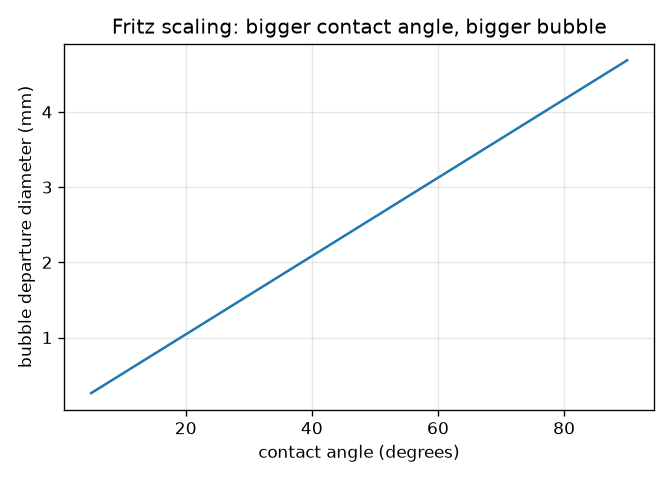
\includegraphics[width=0.85\linewidth]{figures/s02_departure_diameter.png}\\\small Fritz departure diameter against contact angle: proportional, 2.34 mm at 45 degrees.\end{center}

\subsection*{E. Worked example}
Design a kettle element: 1.7 kg of water from 20 C to 100 C in 240 s, element area 100 cm2 (0.01 m2), efficiency 0.85. Find the power, the heat flux, the wall superheat and the safety factor on the CHF (1.1 MW/m2).
\begin{enumerate}[nosep]
\item Energy: Q = 1.7 * 4186 * 80 = 569 296 J (569.3 kJ).
\item Power: P = Q / (eta t) = 569 296 / (0.85 * 240) = 2791 W.
\item Heat flux: q = 0.85 * 2791 / 0.01 = 237 207 W/m2 = 237 kW/m2.
\item Superheat: dT = (q / C)\textasciicircum{}(1/3) = (237 207 / 40.74)\textasciicircum{}(1/3) = 5822\textasciicircum{}(1/3) = 18.0 K, so the wall is at about 118 C.
\item Safety factor: 1.1e6 / 237 207 = 4.6. For a factor of 3 the area could shrink to 3 * 0.85 * 2791 / 1.1e6 = 6.47e-3 m2 = 64.7 cm2.
\end{enumerate}
\textbf{Answer.} About 2.8 kW; the flux is 237 kW/m2, the element runs about 18 K above the water (118 C) and has a safety factor of 4.6 on the critical heat flux.

\subsection*{F. Questions}
\begin{enumerate}[nosep]
\item \textbf{Conceptual.} Why does the heat transfer coefficient h = q / dT increase with the heat flux in nucleate boiling, whereas in natural convection it is roughly constant?
\item \textbf{Numerical.} With the illustrative C = 40.74 W/(m2 K3), the flux at 10 K is 40.7 kW/m2. What is it at 15 K? By what factor does the flux grow when the superheat grows by half?
\item \textbf{Graph and simulation interpretation.} Using the q versus superheat graph, at about what superheat does the flux reach half of the critical heat flux (550 kW/m2)? What does that mean for the wall temperature?
\item \textbf{Design and optimisation challenge.} Design: a 3000 W element must give a safety factor of at least 3 on the CHF and keep the wall below 125 C. What is the smallest area? How long does it take to boil 1.7 kg from 20 C?
\end{enumerate}

\section{Session 3: A heated plate, the burnout and the growing bubble}

\subsection*{A. Real-world problem}
A heater plate sits in water. Turn the power up slowly and the plate stays only a few tens of kelvin above 100 C while the water boils vigorously. Turn it up a little too far and within seconds the plate is far too hot. That is burnout. Can a simple model show why, and why a thermostat that holds the wall temperature instead of the power does not burn out? (Educational model with illustrative coefficients; never use it to test or design real heating equipment.)

\subsection*{B. Concept and theory}
A thin plate of heat capacity C\_p per unit area (J/(m2 K)) is heated by a flux q\_in and cooled by boiling with the flux q(dT): C\_p d(dT)/dt = q\_in - q(dT). The boiling curve q(dT) is piecewise: natural convection h dT, nucleate boiling C dT\textasciicircum{}3 up to the critical heat flux, transition boiling falling (straight on a log scale) to a minimum, and film boiling rising slowly. These pieces and their coefficients are ILLUSTRATIVE: they give the right shape and a peak near 1.1 MW/m2 and are not a correlation fitted to data. In steady state q\_in = q(dT). Below the CHF the nucleate branch has a stable solution: if the plate warms, q rises faster than q\_in and cools it back. Above the CHF no nucleate solution exists: q\_in exceeds the largest flux, the plate keeps warming, passes through the falling transition branch (where warming reduces cooling, a runaway) and lands on the film branch at a far higher temperature. When power is lowered again the plate stays on the film branch until the flux drops to the film minimum: this is hysteresis. If instead the wall temperature is held, the heater supplies whatever q(dT) is, and the curve is walked in either direction without a jump. A bubble grows because liquid near the wall is superheated by dT\_sup; its growth is controlled by heat diffusion into the bubble surface. The Jakob number Ja = rho\_l cp dT\_sup / (rho\_v L) is the ratio of sensible heat in the superheated liquid to the latent heat of the vapour; in a thin thermal layer the radius is R = 2 Ja sqrt(alpha t / pi) (planar), and the classic spherical Plesset-Zwick scaling is R = 2 sqrt(3 / pi) Ja sqrt(alpha t), sqrt(3) times larger. In both, R is proportional to the square root of time.

\begin{itemize}[nosep]
\item dT: wall superheat T\_wall - 100 C (K)
\item q, q\_in: boiling heat flux, supplied heat flux (W/m2)
\item C\_p: plate heat capacity per area (17 250 for 5 mm copper) (J/(m2 K))
\item Q\_chf: critical heat flux (illustrative 1.1e6) (W/m2)
\item surface: scales the nucleate coefficient (1 reference, 0.6 fouled) (no unit)
\item Ja: Jakob number (no unit)
\item alpha: thermal diffusivity of liquid water (1.68e-7) (m2/s)
\item R: bubble radius (m)
\item t: time (s)
\end{itemize}

\begin{equation*}
C_p\,\frac{d(\Delta T)}{dt}=q_{\mathrm{in}}(t)-q(\Delta T)
\end{equation*}

\begin{equation*}
q(\Delta T)=\begin{cases}\max(h\,\Delta T,\ C\,\Delta T^{3}) & \Delta T\le\Delta T_{\mathrm{chf}}\\ \text{log-linear fall to }q_{\min} & \Delta T_{\mathrm{chf}}<\Delta T\le\Delta T_{\min}\\ q_{\min}\,\Delta T/\Delta T_{\min} & \Delta T>\Delta T_{\min}\end{cases}
\end{equation*}

\begin{equation*}
\Delta T(t)=\frac{q_{\mathrm{in}}}{h}\left(1-e^{-h t/C_p}\right)\quad\text{(exact, natural convection only)}
\end{equation*}

\begin{equation*}
\int q_{\mathrm{in}}\,dt-\int q\,dt=C_p\,\Delta T(t_{\mathrm{end}})-C_p\,\Delta T(0)
\end{equation*}

\begin{equation*}
R_{\mathrm{PZ}}=2\sqrt{\tfrac{3}{\pi}}\,\mathrm{Ja}\sqrt{\alpha t},\qquad \mathrm{Ja}=\frac{\rho_l c_p\,\Delta T_{\mathrm{sup}}}{\rho_v L}
\end{equation*}

\begin{center}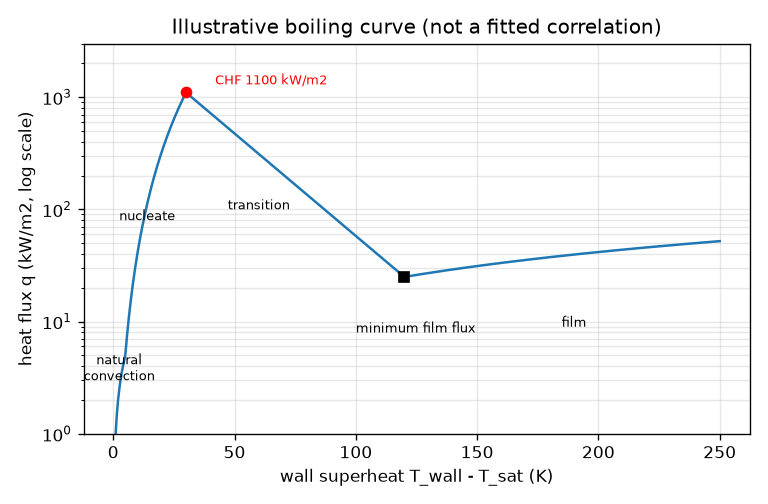
\includegraphics[width=0.85\linewidth]{figures/s03_boiling_curve.png}\\\small Illustrative piecewise boiling curve with its four regimes, critical heat flux and film minimum.\end{center}

\subsection*{E. Worked example}
Apply a heat flux of 600 kW/m2 to the reference plate. Find the steady wall superheat by hand and check it against the simulation; then check the stepper against the exact solution for a constant 3000 W/m2.
\begin{enumerate}[nosep]
\item At steady state q\_in = C dT\textasciicircum{}3 with C = 1.1e6 / 30\textasciicircum{}3 = 40.74 W/(m2 K3).
\item dT = (600 000 / 40.74)\textasciicircum{}(1/3) = 14 727\textasciicircum{}(1/3) = 24.5 K, so the plate is at 124.5 C.
\item Simulation: after a 60 s run with the heat flux ramped in over 10 s, dT = 24.51 K. They agree to 0.01 K.
\item For q\_in = 3000 W/m2 the plate is in natural convection and the exact solution is dT = 3 (1 - exp(-t / 17.25 s)).
\item The stepper's maximum error over 60 s is 0.0002 K; the energy in, out and stored balance to 1e-14 of the input.
\end{enumerate}
\textbf{Answer.} 600 kW/m2 gives a steady superheat of 24.5 K (124.5 C), found by hand and by the simulation; the solver reproduces the exact exponential to 0.0002 K.

\subsection*{F. Questions}
\begin{enumerate}[nosep]
\item \textbf{Conceptual.} Why does a power-controlled heater burn out when the heat flux exceeds the critical heat flux, while a temperature-controlled one does not?
\item \textbf{Numerical.} Use the hand calculation to find the steady superheat for 1000 kW/m2 on the reference surface and for the same flux on the fouled surface (factor 0.6). What happens on the fouled surface?
\item \textbf{Graph and simulation interpretation.} In the hysteresis figure the jump up is at about 1100 kW/m2 and the return at about 13 kW/m2. What does this tell an operator who sees the plate burn out and then reduces the power by 20 percent?
\item \textbf{Design and optimisation challenge.} Design: a 0.04 m2 heater must be safe on a new and a fouled surface with a 20 percent power overshoot, at most 60 percent of the CHF and at most 25 K superheat. Find the largest safe power on a 1 kW grid. Is 60 percent of the CHF alone sufficient?
\end{enumerate}

\section{Real-world mini-project}
\textbf{Choose a safe heater power for a boiling surface.} A flat heater of area 0.04 m2 (200 cm2 square) sits in water at 1 atm. The same heater must stay safe whether its surface is new (surface factor 1.0) or fouled (0.6). Safe means: the heat flux is at most 60 percent of the critical heat flux, the steady wall superheat is at most 25 K on both surfaces, and a 20 percent power overshoot does not burn the plate out in the Session 3 simulation. Use \texttt{design\_check} and \texttt{max\_safe\_power} from Session 3. The coefficients are illustrative, so this is an exercise in method, not a real heater specification.

\section{The path ahead}
\begin{enumerate}[nosep]
\item \textbf{Session 4: Replace the hand-picked curve with correlations.} A boiling curve computed from fluid properties at any pressure.
\item \textbf{Session 5: A spherical bubble in the superheated liquid.} A radial diffusion solver for the growing bubble.
\item \textbf{Session 6: A plate with a temperature profile.} A plate meshed in thickness with boiling as the boundary condition.
\item \textbf{Session 7: From one bubble to a flux.} A bubble-ensemble model that predicts the nucleate flux.
\item \textbf{Session 8: Watch a bubble leave in 2D.} A two-dimensional simulation of a bubble growing, necking and departing.
\end{enumerate}

\section{Answers and hints}

\subsection*{Session 1}
\begin{enumerate}[nosep]
\item \textbf{Conceptual.} Hint: Think about what leaves the pot. Solution: It goes into the latent heat: the energy that turns liquid water into steam. About 2.257 million joules are needed for each kilogram, and the steam carries that energy away. The temperature of boiling water cannot rise at fixed pressure, so all the additional energy becomes vapour, at a rate of eta P / L kilograms per second.
\item \textbf{Numerical.} Hint: Use t = m cp dT / (eta P), then the mass rate eta P / L. Solution: Time = 1.5 * 4186 * 80 / (0.85 * 1800) = 502 320 / 1530 = 328 s (about 5.5 minutes). Then boiled mass = 0.85 * 1800 * 120 / 2.257e6 = 183 600 / 2.257e6 = 0.081 kg = 81 g. Sanity check: 2 minutes of boiling removes only about 5 percent of the water, much less than the 328 s of warming would suggest, because L is 540 times cp.
\item \textbf{Graph and simulation interpretation.} Hint: Use the readout of the boiling-curve view, or the numbers printed by lesson.py. Solution: 10 K: nucleate boiling, about 41 kW/m2. 60 K: transition boiling, about 312 kW/m2 (the largest of the three, but past the peak). 200 K: film boiling, about 38 kW/m2. It is surprising that the surface at 200 K, 190 K hotter, carries about the same heat flux as the one at 10 K: the vapour blanket insulates it. The curve is not monotonic.
\item \textbf{Design and optimisation challenge.} Hint: Solve t = m cp dT / (eta P) for P, then use eta P / L for the mass rate. Solution: P = 334 880 / (0.85 * 180) = 2189 W, so a 2.2 kW heater. Left at that power, the boil-off rate is 0.85 * 2189 / 2.257e6 = 0.82 g/s, so about 495 g in 10 minutes: half the water. Better: turn the power down once boiling starts. To keep a gentle boil you only need enough power to replace the heat losses plus the steam you accept, for example a quarter of the power loses about a quarter as much water. Trade-off: faster start against water loss and energy use. Assumptions: constant efficiency, no lid.
\end{enumerate}

\subsection*{Session 2}
\begin{enumerate}[nosep]
\item \textbf{Conceptual.} Hint: Use q = C dT\textasciicircum{}3 and divide by dT. Solution: From q = C dT\textasciicircum{}3, h = q / dT = C dT\textasciicircum{}2, so h grows with dT and with q. Physically, more heat flux means more bubble sites are active and more bubbles leave per second, and each departing bubble stirs the liquid near the surface and carries away heat. In natural convection there are no bubbles and the flow does not intensify the same way, so h is roughly constant.
\item \textbf{Numerical.} Hint: q is proportional to dT cubed. Solution: q(15) = 40.74 * 15\textasciicircum{}3 = 40.74 * 3375 = 137.5 kW/m2. The factor is 1.5\textasciicircum{}3 = 3.375. Sanity check: the superheat grew by only 5 K while the flux more than tripled; that is why a small rise in wall temperature carries a large rise in power.
\item \textbf{Graph and simulation interpretation.} Hint: Solve 550 000 = 40.74 dT\textasciicircum{}3, or read the curve. Solution: dT = (550 000 / 40.74)\textasciicircum{}(1/3) = 13 500\textasciicircum{}(1/3) = 23.8 K, so the wall is at about 124 C. Half of the critical heat flux is reached at 79 percent of the superheat of the peak (30 K), because of the cube root. The curve is steep: the last 20 percent of superheat gives half of the flux.
\item \textbf{Design and optimisation challenge.} Hint: Two constraints: flux from the safety factor and flux from the superheat limit. Take the more demanding one. Solution: Safety factor 3: q \textless{}= 1.1e6 / 3 = 367 kW/m2, so A \textgreater{}= 0.85 * 3000 / 366 667 = 6.95e-3 m2 = 69.5 cm2. Wall below 125 C: dT \textless{}= 25 K, q \textless{}= 40.74 * 25\textasciicircum{}3 = 636.6 kW/m2, so A \textgreater{}= 2550 / 636 600 = 4.0e-3 m2 = 40.1 cm2. The safety factor is the binding constraint: A \textgreater{}= 69.5 cm2. Time to boil: 569 296 / (0.85 * 3000) = 223 s. Trade-off: a bigger element costs more and is harder to fit, but gives a larger margin and a cooler wall. Assumption: uniform flux and the illustrative coefficient.
\end{enumerate}

\subsection*{Session 3}
\begin{enumerate}[nosep]
\item \textbf{Conceptual.} Hint: Compare q\_in = q(dT) with the shape of the boiling curve past the peak. Solution: Above the CHF no nucleate-boiling state can carry the supplied flux: the plate warms, enters transition boiling where a higher temperature means a lower flux, so cooling falls as heating continues, and it runs away to the film-boiling branch at a far higher temperature. A temperature-controlled heater sets dT, so the heat flux is whatever the boiling curve gives, whatever the shape; the control reduces the supplied power if the flux falls, so there is nothing to run away.
\item \textbf{Numerical.} Hint: dT = (q / (C surface))\textasciicircum{}(1/3), with C = 40.74. Solution: Reference: (1.0e6 / 40.74)\textasciicircum{}(1/3) = 29.1 K. Fouled: C = 24.44, dT = (1.0e6 / 24.44)\textasciicircum{}(1/3) = 34.5 K. The critical heat flux is still 1.1 MW/m2 (the peak is now at 35.6 K), so it stays below the peak but the wall runs 5 K hotter and the margin to the peak is thin. Units: kelvin above 100 C, so about 129 C and 135 C.
\item \textbf{Graph and simulation interpretation.} Hint: Where is the plate sitting on the curve after the jump? Solution: The plate is now on the film-boiling branch and stays there until the flux falls to the order of the film minimum, about 25 kW/m2 (13 kW/m2 in the simulation, which lags because the plate takes time to cool). A 20 percent reduction brings the flux to about 880 kW/m2, about 70 times higher than the return flux, so the plate stays burned out. The operator must remove nearly all of the power, not just back off a little.
\item \textbf{Design and optimisation challenge.} Hint: Use design\_check(P, 0.04) for P from 14 to 27 kW. Solution: The 60 percent limit alone allows a flux of 660 kW/m2, i.e. 26.4 kW, but at 26 kW the fouled surface runs 29.8 K above boiling, above the 25 K limit. The largest safe power on the grid is 15 kW: a flux of 375 kW/m2 gives 21.0 K (new) and 24.8 K (fouled). 16 kW gives 25.4 K on the fouled surface and fails. A 20 percent overshoot (450 kW/m2) is far below the CHF so it does not burn out. Trade-off: the superheat limit on a fouled surface governs the design, not the CHF. The constants are illustrative, so this is a method, not a specification.
\end{enumerate}

\section{How to join}
Read \texttt{CONTRIBUTING.md} in the repository, then pick an issue labelled \texttt{good first issue}. Repository: \url{https://github.com/KrunalPanchal1995/openboiling}

\end{document}
